\documentclass[letterpaper,11pt]{article}

% Soporte para los acentos.
\usepackage[utf8]{inputenc}
\usepackage[T1]{fontenc}
% Idioma español.
\usepackage[spanish,mexico, es-tabla]{babel}
% Soporte de símbolos adicionales (matemáticas)
\usepackage{multirow}
\usepackage{amsmath}
\usepackage{amssymb}
\usepackage{amsthm}
\usepackage{amsfonts}
\usepackage{mathtools}
\usepackage{latexsym}
\usepackage{enumerate}
\usepackage{ragged2e}
\usepackage{listings}
\usepackage[dvipsnames]{xcolor}
\usepackage{multicol}
\usepackage{wrapfig,lipsum,booktabs}
\usepackage{float}
\usepackage{graphicx}
\usepackage{subcaption}
\usepackage{hyperref}
\usepackage[linguistics]{forest}
\usetikzlibrary{positioning,matrix, arrows.meta}

% Modificamos los márgenes del documento.                                       
\usepackage[lmargin=1.5cm,rmargin=1.5cm,top=1.5cm,bottom=1.5cm]{geometry}

\title{Facultad de Ciencias, UNAM \\ 
       Análisis de Algoritmos \\ 
       Tarea 3}
\author{Rubí Rojas Tania Michelle}
\date{11 de diciembre de 2020}

\begin{document}
\maketitle

\begin{enumerate}
    % Ejercicio 1.
    \item Un pescador está sobre un océano rectangular. El valor del pez en el 
    punto $(i, j)$ está dado por un arreglo $A$ de dimensión $2 (n \times m)$.
    Diseña un algoritmo que calcule el máximo valor de pescado que un pescador
    puede atrapar en un camino desde la esquina superior izquierda a la esquina 
    inferior derecha. El pescador sólo puede moverse hacia abajo o hacia arriba,
    como se ilustra en la siguiente figura: 
    \begin{figure}[h]
        \centering
        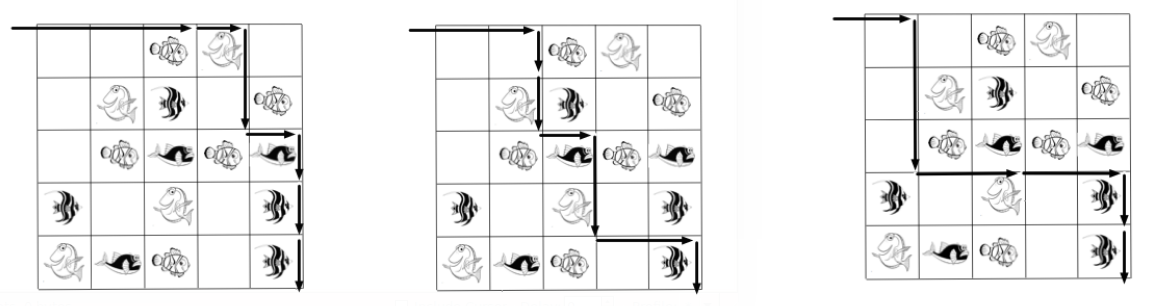
\includegraphics[width=0.5\linewidth]{imagenes/ejercicio1.png}
    \end{figure}

    % Ejercicio 2.
    \item Dados dos árboles generadores $T$ y $R$ de una gráfica $G$. Muestra 
    cómo encontrar la secuencia más corta de árboles generadores $T_0, T_1, 
    \ldots, T_k$ tal que $T_0 = T, T_k = R$, y cada árbol $T_i$ difiere del 
    anterior $T_{i-1}$ agregando y borrando una arista.

    % Ejercicio 3.
    \item Sea $G$ una gráfica con $n$ vértices. Un subconjunto $S$ de los 
    vértices de $G$ es independiente si cualesquiera dos elementos de $S$ no 
    son adyacentes. En general, el problema de encontrar el conjunto 
    independiente de una gráfica es un problema $NP-$completo. Pero en 
    algunos casos, este problema puede resolverse eficientemente. Sea $T$ un
    árbol con raíz con $n$ vértices. Cada nodo $v \in T$ tiene asociado un peso 
    $w(v)$. Utilizándo programación dinámica, encuentre un algoritmo de tiempo 
    lineal para encontrar el conjunto independiente de $T$ de peso máximo.

    % Ejercicio 4.
    \item Mientras caminas por la playa encuentras un cofre de tesoros. El 
    cofre contiene $n$ tesoros con pesos $w_i, \ldots, w_n$ y valores 
    $v_1, \ldots, v_n$. Desafortunadamente, sólo tienes una maleta que sólo 
    tiene capacidad de carga $M$. Afortunadamente, los tesoros se pueden romper
    si es necesario. Por ejemplo, la tercera parte de un tesoro $i$ tiene peso
    $\frac{w_i}{3}$ y valor $\frac{v_i}{3}$.
    \begin{itemize}
        % Ejercicio 4.a
        \item Describe un algoritmo voraz de tiempo $\theta(n \log n)$ que 
        resuelve este problema.

        \textsc{Solución:}

        % Ejercicio 4.b
        \item ¿Se puede mejorar el tiempo de ejecución de tu algoritmo a 
        $\theta(n)$? Si es un no, explica por qué; si es un sí, menciona el 
        cambio.
    \end{itemize}

    % Ejercicio 5.
    \item Un grupo de personas quiere comprar un ramo de flores, y el florista
    que las vende quiere maximizar sus ganancias al venderlas. Para esto ha 
    decidido determinar el precio de las flores que cada cliente compra como
    sigue: el precio de su primer flor será $(0 + 1) \times c$, donde $c$ es 
    el precio original de la flor; el costo de la segunda flor será $(1 + 1)
    \times c$, y así sucesivamente. Dado un grupo de $n$ personas, un número 
    $n$ de flores que desean comprar, y el costo original $c$ de las flores, 
    diseñe un algoritmo que en tiempo $O(n \log n)$ minimice el costo total 
    que los clientes tienen que pagar para que entre todos compren todas las 
    flores. 

    % Ejercicio 6.
    \item Sean $k, n \in \mathbb{N}$. El problema de los huevos, es el 
    siguiente: tenemos un edificio con $n$ pisos y $k$ huevos. Sabemos que hay 
    un piso $f$ tal que si dejamos caer un huevo desde el piso $f$, se 
    estrellará. Si dejamos caer un huevo desde un piso $r$ tal que $r < f$, el 
    huevo no se estrellará, y si dejamos caer el huevo desde un piso 
    $r \geq f$, el huevo se estrellará (es posible que $f = 1$, en cuyo caso, 
    el huevo siempre se estrellará. Si $f = n+1$, el huevo nunca se estrellará).
    \textbf{Una vez que un huevo se estrella, no lo podemos usar nuevamente}. 
    Si disponemos de $k$ huevos, ¿cuál es el menor número de experimentos
    (dejar caer un huevo) que se tienen que hacer para determinar a $f$? Sea 
    $E(k, n)$ el mínimo número de experimentos que tiene que hacer para 
    determinar a $f$.
    \begin{enumerate}
        % Ejercicio 6.a
        \item Pruebe que $E(1, n) = n$.

        % Ejercicio 6.b
        \item Encuentre una recurrencia para $E(k,n)$. Utilice programación 
        dinámica para encontrar $E(k,n)$. ¿Qué tan rápido es su algoritmo?
    \end{enumerate}

    % Ejercicio 7.
    \item Construye el árbol de Huffman para codificar el siguiente texto:
    \begin{center}
        \textit{"La rabia es como el picante. Una pizca te despierta, pero
        en exceso te adormece"}
    \end{center}
    
    \textsc{Solución:} Primero, ignorándo mayúsculas, vamos a crear una tabla 
    de frecuencias para los símbolos y letras en nuestro texto
    \begin{figure}[H]
        \centering
        \begin{tabular}{|c|c|}
            \hline
            símbolo & frecuencia \\
            \hline
            b & 1 \\
            \hline
            u & 1 \\
            \hline
            x & 1 \\
            \hline
            z & 1 \\
            \hline
            . & 1 \\
            \hline
            , & 1 \\
            \hline
            d & 2 \\
            \hline
            l & 2 \\
            \hline
            m & 2 \\
            \hline
            n & 3 \\
            \hline
            s & 3 \\
            \hline
            i & 4 \\
            \hline
            p & 4 \\
            \hline
            r & 4 \\
            \hline
            t & 4 \\
            \hline
            c & 5 \\
            \hline
            o & 5 \\
            \hline
            a & 8 \\
            \hline
            e & 13 \\
            \hline
            \texttt{\char32} & 14 \\
            \hline
        \end{tabular}
        \caption{Tabla de frecuencias ordenada}
    \end{figure}

    Luego, realizaremos las actualizaciones de la tabla de frecuencias:
    \begin{table}[h]
        \parbox{.45\linewidth}{
        \centering
        \begin{tabular}{|c|c|}
            \hline
            símbolo & frecuencia \\
            \hline
            x & 1 \\
            \hline
            z & 1 \\
            \hline
            . & 1 \\
            \hline
            , & 1 \\
            \hline
            bu & 2 \\
            \hline
            d & 2 \\
            \hline
            l & 2 \\
            \hline
            m & 2 \\
            \hline
            n & 3 \\
            \hline
            s & 3 \\
            \hline
            i & 4 \\
            \hline
            p & 4 \\
            \hline
            r & 4 \\
            \hline
            t & 4 \\
            \hline
            c & 5 \\
            \hline
            o & 5 \\
            \hline
            a & 8 \\
            \hline
            e & 13 \\
            \hline
            \texttt{\char32} & 14 \\
            \hline
        \end{tabular}
        \caption{Unimos los símbolos \texttt{b} y \texttt{u}}
        }
        \hfill
        \parbox{.45\linewidth}{
        \centering
        \begin{tabular}{|c|c|}
            \hline
            símbolo & frecuencia \\
            \hline
            . & 1 \\
            \hline
            , & 1 \\
            \hline
            bu & 2 \\
            \hline
            xz & 2 \\
            \hline
            d & 2 \\
            \hline
            l & 2 \\
            \hline
            m & 2 \\
            \hline
            n & 3 \\
            \hline
            s & 3 \\
            \hline
            i & 4 \\
            \hline
            p & 4 \\
            \hline
            r & 4 \\
            \hline
            t & 4 \\
            \hline
            c & 5 \\
            \hline
            o & 5 \\
            \hline
            a & 8 \\
            \hline
            e & 13 \\
            \hline
            \texttt{\char32} & 14 \\
            \hline
        \end{tabular}
        \caption{Unimos los símbolos \texttt{x} y \texttt{z}}
        }
    \end{table}

    \begin{table}[H]
        \parbox{.45\linewidth}{
        \centering
        \begin{tabular}{|c|c|}
            \hline
            símbolo & frecuencia \\
            \hline
            bu & 2 \\
            \hline
            xz & 2 \\
            \hline
            ., & 2 \\
            \hline
            d & 2 \\
            \hline
            l & 2 \\
            \hline
            m & 2 \\
            \hline
            n & 3 \\
            \hline
            s & 3 \\
            \hline
            i & 4 \\
            \hline
            p & 4 \\
            \hline
            r & 4 \\
            \hline
            t & 4 \\
            \hline
            c & 5 \\
            \hline
            o & 5 \\
            \hline
            a & 8 \\
            \hline
            e & 13 \\
            \hline
            \texttt{\char32} & 14 \\
            \hline
        \end{tabular}
        \caption{Unimos los símbolos \texttt{.} y \texttt{,}}
        }
        \hfill
        \parbox{.45\linewidth}{
        \centering
        \begin{tabular}{|c|c|}
            \hline
            símbolo & frecuencia \\
            \hline
            ., & 2 \\
            \hline
            d & 2 \\
            \hline
            l & 2 \\
            \hline
            m & 2 \\
            \hline
            n & 3 \\
            \hline
            s & 3 \\
            \hline
            buxz & 4 \\
            \hline
            i & 4 \\
            \hline
            p & 4 \\
            \hline
            r & 4 \\
            \hline
            t & 4 \\
            \hline
            c & 5 \\
            \hline
            o & 5 \\
            \hline
            a & 8 \\
            \hline
            e & 13 \\
            \hline
            \texttt{\char32} & 14 \\
            \hline
        \end{tabular}
        \caption{Unimos los símbolos \texttt{bu} y \texttt{xz}}
        }
    \end{table}

    \begin{table}[H]
        \parbox{.45\linewidth}{
        \centering
        \begin{tabular}{|c|c|}
            \hline
            símbolo & frecuencia \\
            \hline
            l & 2 \\
            \hline
            m & 2 \\
            \hline
            n & 3 \\
            \hline
            s & 3 \\
            \hline
            buxz & 4 \\
            \hline
            .,d & 4 \\
            \hline
            i & 4 \\
            \hline
            p & 4 \\
            \hline
            r & 4 \\
            \hline
            t & 4 \\
            \hline
            c & 5 \\
            \hline
            o & 5 \\
            \hline
            a & 8 \\
            \hline
            e & 13 \\
            \hline
            \texttt{\char32} & 14 \\
            \hline
        \end{tabular}
        \caption{Unimos los símbolos \texttt{.,} y \texttt{d}}
        }
        \hfill
        \parbox{.45\linewidth}{
        \centering
        \begin{tabular}{|c|c|}
            \hline
            símbolo & frecuencia \\
            \hline
            n & 3 \\
            \hline
            s & 3 \\
            \hline
            buxz & 4 \\
            \hline
            .,d & 4 \\
            \hline
            lm & 4 \\
            \hline
            i & 4 \\
            \hline
            p & 4 \\
            \hline
            r & 4 \\
            \hline
            t & 4 \\
            \hline
            c & 5 \\
            \hline
            o & 5 \\
            \hline
            a & 8 \\
            \hline
            e & 13 \\
            \hline
            \texttt{\char32} & 14 \\
            \hline
        \end{tabular}
        \caption{Unimos los símbolos \texttt{l} y \texttt{m}}
        }
    \end{table}

    \begin{table}[H]
        \parbox{.45\linewidth}{
        \centering
        \begin{tabular}{|c|c|}
            \hline
            símbolo & frecuencia \\
            \hline
            buxz & 4 \\
            \hline
            .,d & 4 \\
            \hline
            lm & 4 \\
            \hline
            i & 4 \\
            \hline
            p & 4 \\
            \hline
            r & 4 \\
            \hline
            t & 4 \\
            \hline
            c & 5 \\
            \hline
            o & 5 \\
            \hline
            ns & 6 \\
            \hline
            a & 8 \\
            \hline
            e & 13 \\
            \hline
            \texttt{\char32} & 14 \\
            \hline
        \end{tabular}
        \caption{Unimos los símbolos \texttt{n} y \texttt{s}}
        }
        \hfill
        \parbox{.45\linewidth}{
        \centering
        \begin{tabular}{|c|c|}
            \hline
            símbolo & frecuencia \\
            \hline
            lm & 4 \\
            \hline
            i & 4 \\
            \hline
            p & 4 \\
            \hline
            r & 4 \\
            \hline
            t & 4 \\
            \hline
            c & 5 \\
            \hline
            o & 5 \\
            \hline
            ns & 6 \\
            \hline
            buxz.,d & 8 \\
            \hline
            a & 8 \\
            \hline
            e & 13 \\
            \hline
            \texttt{\char32} & 14 \\
            \hline
        \end{tabular}
        \caption{Unimos los símbolos \texttt{buxz} y \texttt{.,d}}
        }
    \end{table}

    \begin{table}[H]
        \parbox{.45\linewidth}{
        \centering
        \begin{tabular}{|c|c|}
            \hline
            símbolo & frecuencia \\
            \hline
            p & 4 \\
            \hline
            r & 4 \\
            \hline
            t & 4 \\
            \hline
            c & 5 \\
            \hline
            o & 5 \\
            \hline
            ns & 6 \\
            \hline
            buxz.,d & 8 \\
            \hline
            lmi & 8 \\
            \hline
            a & 8 \\
            \hline
            e & 13 \\
            \hline
            \texttt{\char32} & 14 \\
            \hline
        \end{tabular}
        \caption{Unimos los símbolos \texttt{lm} y \texttt{i}}
        }
        \hfill
        \parbox{.45\linewidth}{
        \centering
        \begin{tabular}{|c|c|}
            \hline
            símbolo & frecuencia \\
            \hline
            t & 4 \\
            \hline
            c & 5 \\
            \hline
            o & 5 \\
            \hline
            ns & 6 \\
            \hline
            buxz.,d & 8  \\
            \hline
            lmi & 8 \\
            \hline
            pr & 8 \\
            \hline
            a & 8 \\
            \hline
            e & 13 \\
            \hline
            \texttt{\char32} & 14 \\
            \hline
        \end{tabular}
        \caption{Unimos los símbolos \texttt{p} y \texttt{r}}
        }
    \end{table}

    \begin{table}[H]
        \parbox{.45\linewidth}{
        \centering
        \begin{tabular}{|c|c|}
            \hline
            símbolo & frecuencia \\
            \hline
            o & 5 \\
            \hline
            ns & 6 \\
            \hline
            buxz.,d & 8 \\
            \hline
            lmi & 8 \\
            \hline
            pr & 8 \\
            \hline
            a & 8 \\
            \hline
            tc & 9 \\
            \hline
            e & 13 \\
            \hline
            \texttt{\char32} & 14 \\
            \hline
        \end{tabular}
        \caption{Unimos los símbolos \texttt{t} y \texttt{c}}
        }
        \hfill
        \parbox{.45\linewidth}{
        \centering
        \begin{tabular}{|c|c|}
            \hline
            símbolo & frecuencia \\
            \hline
            buxz.,d & 8 \\
            \hline
            lmi & 8 \\
            \hline
            pr & 8 \\
            \hline
            a & 8 \\
            \hline
            tc & 9 \\
            \hline
            ons & 11 \\
            \hline
            e & 13 \\
            \hline
            \texttt{\char32} & 14 \\
            \hline
        \end{tabular}
        \caption{Unimos los símbolos \texttt{o} y \texttt{ns}}
        }
    \end{table}

    \begin{table}[H]
        \parbox{.45\linewidth}{
        \centering
        \begin{tabular}{|c|c|}
            \hline
            símbolo & frecuencia \\
            \hline
            pr & 8 \\
            \hline
            a & 8 \\
            \hline
            tc & 9 \\
            \hline
            ons & 11 \\
            \hline
            e & 13 \\
            \hline
            \texttt{\char32} & 14 \\
            \hline
            buxz.,dlmi&  16 \\
            \hline
        \end{tabular}
        \caption{Unimos los símbolos \texttt{buxz.,d} y \texttt{lmi}}
        }
        \hfill
        \parbox{.45\linewidth}{
        \centering
        \begin{tabular}{|c|c|}
            \hline
            símbolo & frecuencia \\
            \hline
            tc & 9 \\
            \hline
            ons & 11 \\
            \hline
            e & 13 \\
            \hline
            \texttt{\char32} & 14 \\
            \hline
            buxz.,dlmi&  16\\
            \hline
            pra & 16 \\
            \hline
        \end{tabular}
        \caption{Unimos los símbolos \texttt{pr} y \texttt{a}}
        }
    \end{table}

    \begin{table}[H]
        \parbox{.45\linewidth}{
        \centering
        \begin{tabular}{|c|c|}
            \hline
            símbolo & frecuencia \\
            \hline
            e & 13 \\
            \hline
            \texttt{\char32} & 14 \\
            \hline
            buxz.,dlmi&  16 \\
            \hline
            pra & 16\\
            \hline
            tcons & 20 \\
            \hline
        \end{tabular}
        \caption{Unimos los símbolos \texttt{tc} y \texttt{ons}}
        }
        \hfill
        \parbox{.45\linewidth}{
        \centering
        \begin{tabular}{|c|c|}
            \hline
            símbolo & frecuencia \\
            \hline
            buxz.,dlmi & 16 \\
            \hline
            pra & 16 \\
            \hline
            tcons & 20 \\
            \hline
            e \texttt{\char32} & 27 \\
            \hline
        \end{tabular}
        \caption{Unimos los símbolos \texttt{e} y \texttt{\char32}}
        }
    \end{table}

    \begin{table}[H]
        \parbox{.45\linewidth}{
        \centering
        \begin{tabular}{|c|c|}
            \hline
            símbolo & frecuencia \\
            \hline
            tcons & 20 \\
            \hline
            e \texttt{\char32} & 27 \\
            \hline
            buxz.,dlmipra & 32\\
            \hline
        \end{tabular}
        \caption{Unimos los símbolos \texttt{buxz.,dlmi} y \texttt{pra}}
        }
        \hfill
        \parbox{.45\linewidth}{
        \centering
        \begin{tabular}{|c|c|}
            \hline
            símbolo & frecuencia \\
            \hline
            buxz$\cdot \mathbin{,}$dlmipra & 32 \\
            \hline
            tconse \texttt{\char32} & 47 \\
            \hline
        \end{tabular}
        \caption{Unimos los símbolos \texttt{tcons} y \texttt{e \char32}}
        }
    \end{table}

    \begin{table}[H]
        \parbox{.45\linewidth}{
        \centering
        \begin{tabular}{|c|c|}
        \hline
        buxz$\cdot \mathbin{,}$dlmipransotce \texttt{\char32} & 79\\
        \hline
        \end{tabular}
        \caption{Unimos los símbolos \texttt{buxz.,dlmipra} y \texttt{tconse \char32}}
        }
    \end{table}
    
    Así, el árbol de Huffman se vería de la forma:
    \begin{figure}[H]
        \centering
        \begin{forest}
        [79 \\ buxz$\cdot \mathbin{,}$dlmipransotce \texttt{\char32}
          [32 \\ buxz$\cdot \mathbin{,}$dlmipra, edge label={node[midway,left,font=\scriptsize]{0\;\;\;\;\;\;\;}}
            [16 \\ buxz$\cdot \mathbin{,}$dlmi, edge label={node[midway,left,font=\scriptsize]{0\;\;\;\;}}
              [8 \\ buxz $\cdot \mathbin{,}$d, edge label={node[midway,left,font=\scriptsize]{0\;\;\;}}
                [4 \\ buxz, edge label={node[midway,left,font=\scriptsize]{0\;\;}}
                  [2 \\ bu, edge label={node[midway,left,font=\scriptsize]{0\;}} 
                    [1 \\ b, blue, edge label={node[midway,left,font=\scriptsize]{0}}] 
                    [1 \\ u, blue, edge label={node[midway,right,font=\scriptsize]{1}}]] 
                  [2 \\ xz, edge label={node[midway,right,font=\scriptsize]{\;1}}
                    [1 \\ x, blue, edge label={node[midway,left,font=\scriptsize]{0}}] 
                    [1 \\ z, blue, edge label={node[midway,right,font=\scriptsize]{1}}]]] 
                [4 \\ $\cdot \mathbin{,}$d, edge label={node[midway,right,font=\scriptsize]{\;\;1}}
                  [2 \\ $\cdot \mathbin{,}$, edge label={node[midway,left,font=\scriptsize]{0\;}}
                    [1 \\ $\cdot$, blue, edge label={node[midway,left,font=\scriptsize]{0}}] 
                    [1 \\ $\mathbin{,}$, blue, edge label={node[midway,right,font=\scriptsize]{1}}]] 
                [2 \\ d, blue, edge label={node[midway,right,font=\scriptsize]{1}}]]] 
              [8 \\ lmi, edge label={node[midway,right,font=\scriptsize]{\;\;\;1}}
                [4 \\ lm, edge label={node[midway,left,font=\scriptsize]{0}}
                  [2 \\ l, blue, edge label={node[midway,left,font=\scriptsize]{0}}] 
                  [2 \\ m, blue, edge label={node[midway,right,font=\scriptsize]{1}}]] 
                [4 \\ i, blue, edge label={node[midway,right,font=\scriptsize]{1}}]]]
            [16 \\ pra, edge label={node[midway,right,font=\scriptsize]{\;\;\;\;1}}
              [8 \\ pr, edge label={node[midway,left,font=\scriptsize]{0}}
                [4 \\ p, blue, edge label={node[midway,left,font=\scriptsize]{0}}] 
                [4 \\ r, blue, edge label={node[midway,right,font=\scriptsize]{1}}]] 
              [8 \\ a, blue, edge label={node[midway,right,font=\scriptsize]{1}}]]] 
          [47 \\ tconse \texttt{\char32}, edge label={node[midway,right,font=\scriptsize]{\;\;\;\;\;\;\;1}}
            [20 \\ tcons, edge label={node[midway,left,font=\scriptsize]{0\;\;}}
              [9 \\ tc, edge label={node[midway,left,font=\scriptsize]{0\;}}
                [4 \\ t, blue, edge label={node[midway,left,font=\scriptsize]{0}}] 
                [5 \\ c, blue, edge label={node[midway,right,font=\scriptsize]{1}}]] 
              [11 \\ ons, edge label={node[midway,right,font=\scriptsize]{\;1}}
                [5 \\ o, blue, edge label={node[midway,left,font=\scriptsize]{0}}] 
                [6 \\ ns, edge label={node[midway,right,font=\scriptsize]{1}}
                  [3 \\ n, blue,edge label={node[midway,left,font=\scriptsize]{0}}] 
                  [3 \\ s, blue,edge label={node[midway,right,font=\scriptsize]{1}}]]]] 
            [27 \\ e \texttt{\char32}, edge label={node[midway,right,font=\scriptsize]{\;\;1}}
              [13 \\ e, blue, edge label={node[midway,left,font=\scriptsize]{0}}] 
              [14 \\ \texttt{\char32}, blue, edge label={node[midway,right,font=\scriptsize]{1}}]]]]
        \end{forest}
        \caption{Árbol de Huffman}
    \end{figure}

    Por lo tanto, la codificación de cada símbolo sería
    \begin{center}
        \begin{tabular}{|c|c|}
            \hline
            símbolo & codificación \\
            \hline
            b & 000000\\
            \hline
            u & 000001\\
            \hline
            x & 000010\\
            \hline
            z & 000011\\
            \hline
            $\cdot$ & 000100\\
            \hline
            $\mathbin{,}$ & 000101\\
            \hline
            d & 00011\\
            \hline
            l & 00100\\
            \hline
            m & 00101\\
            \hline
            i & 0011\\
            \hline
            p & 0100\\
            \hline
            r & 0101\\
            \hline
            a & 011 \\
            \hline
            t & 1000\\
            \hline
            c & 1001\\
            \hline
            o & 1010 \\
            \hline
            n & 10110 \\
            \hline
            s & 10111 \\
            \hline
            e & 110 \\
            \hline
            \texttt{\char32} & 111 \\
            \hline
        \end{tabular}
    \end{center}

    % Ejercicio 8.
    \item Supongamos que el mago Merlín tiene un conjunto $A[1, \ldots, n]$ de 
    pociones, las cuales puede mezclar de dos maneras consecutivas con un costo 
    de $A[i] \times A[i + 1]$ y resulta en la poción $A[i] + A[i+1]$. Merlín 
    quiere mezclar todas las pociones pero con el mínimo costo.
    \begin{enumerate}
        % Ejercicio 8.a
        \item Diseña un algoritmo que garantice unir todas las pociones con 
        un costo mínimo.
        
        % Ejercicio 8.b
        \item ¿Cuál es el mínimo costo si se tienen 5 pociones cuyos valores son:
        $1, 9, 6, 2 3$?
    \end{enumerate}

\end{enumerate}

\end{document}
